\section{Discussion}

\subsection{RQ 1: Can user-reported logs help debug production failures?} \label{discussion_rq1}
	
	\subsubsection{Motivation}~ \label{rq1_motivation}

		In the recent years, there are many different techniques to enhance bug localization. However, many of those techniques experience performance overhead when dealing with large-scale systems. Thus, we want to investigate a light-weighted approach that could help developers pinpoint the problematic code. Our work consists of an empirical study on production bug to further research how can we use user-attached logs to localize the bug. Fundamentally, we want to know how helpful are user-reported logs in the event of production failures. As the result of this study, we confirm the usefulness of user-reported logs in bug localization.
	~\\
	
	\subsubsection{Approach}~ \label{rq1_approach}

		By analyzing the user-reported logs, we propose a static analysis approach that automatically recovers the partial system execution that triggered the bug. The main methodology is break down into three steps:
		\vspace{-0.1cm}
		\begin{itemize} \itemsep 0em
		 \item Log Messages Mining
		 \item Log message mapping to logging line
		 \item Call graph construction
		\end{itemize}

		\phead{Overview of our Approach} We first retrieve the log messages from the bug report using regular expression. Then, we leverage static analysis technique to map each log message to its corresponding logging line in source code. Based on on this log message mapping, we traverse through the logging lines to derive a list of potential code paths. We build a control flow graph (e.g., call graph) to represent the partial execution of the system. This identifies the potential problematic code area. Finally, to evaluate the effectiveness of our approach, we will examine the overlaps between bug fix and recovered system execution.
		
		\phead{Project selection} For our case study, we have selected five large-scale open-source Java projects: Hadoop, Hive, Camel, ActiveMQ and Zookeeper. The infrastructures involved in this study vary from virtual machine deployment to data warehouse. To come up with these 5 Java projects, we have done a preliminary study across 16 Apache Software Foundation open-source projects. There are two reasons that push us to select projects from Apache Software Foundation: 1) having access to most of its code base, version control and issue tracker; 2) the development process of those projects is stable, and many of them are actively maintained. As our empirical study focuses on log messages manipulation, we decide to proceed with five projects that contain the most bug reports with logs. We present the result of this preliminary study in Table \ref{table:1}. \verb\BRWL\ abbreviation refers to bug report with log. \verb\BR\ refers to bug report. We calculated the percentage of bug report with log in \verb\%BRWL/BR\. Despite the fact that only a small portion of the reporters attach logs in bug reports (varying between 0.21\% and 8.45\%), our study will focus on the effectiveness of the approach. To better understand the application of our approach in real-world practice, future work will investigate the impact of this low percentage.
		 
		\begin{table}[h!]
	\centering
	\begin{tabular}{||c c c c||} 
	 \hline
		 Project   & BRWL       & BR 	   & \% BRWL/BR \\ [0.5ex] 
		 \hline\hline
		 ActiveMQ  & 201        & 4 590    & 4.38\% \\
		 Camel     & 9 		    & 4 275	   & 0.21\% \\
		 Hadoop    & 781 	    & 20 893   & 3.74\% \\ 
		 Hive 	   & 208 	    & 11 479   & 1.81\% \\
		 Storm 	   & 116	    & 1 507     & 7.70\% \\
		 Zookeeper & 151        & 1 788     & 8.45\% \\ [1ex]
	 \hline
	\end{tabular}
	\caption{Preliminary study on the amount of bug report with logs per project}
\label{table:1}
\end{table}

		Through the investigation, we also discovered some interesting findings. For instance, the majority of user-reported logs are attached directly in \textit{Description} section of the bug report. Table \ref{table:2} illustrates the percentage of bug reports which logs are attached in \textit{Description} section.

		\begin{table}[h!]
	\centering
	\begin{tabular}{||c c c c||} 
	 \hline
		 Project   & BRWL in Desc 		  	   & BRWL 	  & \% BRWL in Desc \\ [0.5ex] 
		 \hline\hline
		 ActiveMQ  & 152     				   & 201      & 75.62\% \\
		 Camel     & 9      				   & 9	  	  & 100\%   \\
		 Hadoop    & 536     				   & 781  	  & 68.63\% \\ 
		 Hive 	   & 62     				   & 208 	  & 29.81\% \\
		 Storm 	   & 106     				   & 116 	  & 91.38\% \\
		 Zookeeper & 152     				   & 151      & 64.90\% \\ [1ex]
	 \hline
	\end{tabular}
	\caption{Percentage of bug reports in which logs are attached in \textit{Description} section}
\label{table:2}
\end{table}

		\phead{Log messages mining} In this step, we want to retrieve all log messages from its corresponding bug report. As Apache Software Foundation hosts its issue tracker on Jira, we first extracted all bug reports through Jira REST APIs. We built a small web application to filter and display the issues. We filtered the issues from a specific set of criteria: 1) Type of issue = Bug 2) Status = CLOSED 3) Created date = within the last 4 years 4) Assignee is different than the reported 5) Resolution = Fixed. Those characteristics are crucial for our study. The issue must be a bug report that was reported within the last 4 years, so we can conduct our analysis on the changes that happened recently. The status and resolution of the issue must be closed and fixed to ensure 1) it is indeed a bug, 2) a solution is furnished. The solution to the bug(e.g., bug fixing commit) added by the assignee will served as our ground truth, to later evaluate our approach. Once we have refined our bug reports set, we use regular expression (e.g., \textit{(?<level>(INFO|ERROR|WARN|TRACE|DEBUG|FATAL)}) to extract the log messages. The following lines shows an example of log messages extracted from Hadoop HDFS, issue number HDFS-2726:
	~\\

		\texttt{
			08/09/09 03:28:36 INFO dfs.DFSClient: Exception in createBlockOutputStream java.io.IOException: Could not read from stream 
			~\\~\\
			\indent 08/09/09 03:28:36 INFO dfs.DFSClient: Abandoning block blk\_624229997631234952\_8205908
		}
	~\\

		\phead{Log message mapping to logging line} After obtaining the log messages, we map the log message to the logging code. We first extract all logging code from the source code using regular expression (e.g., \verb\(?<level>INFO|ERROR|WARN|TRACE|DEBUG|FATAL)\). For each log statement extracted from the source code, we record its package name, file name, line number and the method in which it is called. The records are sent in form of JSON documents to Elasticsearch using its Java API. From there, we use Elasticsearch as our logging line search engine. Elasticsearch is well-known for its high performance nature and able to process large volumes of data in parallel, thus it is perfectly suitable for our study. In order to map log message to its corresponding logging line, we deloyed phrase match strategy. A log message find its match when the later contains all the words appearing in the message; or a close variants from the keyword in the same order. For instance, if we were to match the previous mentionned log message
		\textcolor{blue}{
			\texttt{
				08/09/09 03:28:36 INFO dfs.DFSClient: Exception in createBlockOutputStream java.io.IOException: Could not read from stream
			}
		} to its corresponding logging line, the algorithm will break the message into a set of ordered keywords, the logging line with the most keyword present in the defined order will trigger a match. In this illustrated example, the log message successfully matched with the logging line 
		\textcolor{blue}{
			\texttt{
				DFSClient.LOG.info("Exception in createBlockOutputStream " + ie);
			}
		}
		Although in the perfect scenario, developer should follow good software practice and avoid duplicated logging statements, we have noticed a few cases where more than one identical logging lines are matched. To address this issue, we propose to query the code surronding the logging line. Based on the queried keywords, we can look for the one that contain contexual information hints and differentiate the logging statements. 

		\phead{Call graph construction} In order to build a graph representation of paths traversed by the partial execution, we implemented a static analysis tool based on JavaParser, an open source Abstract Syntax Tree (AST) parser for Java. The JavaParser project helps us to parse Java code into an AST. This structured representation makes the code easier to process. If we want to find the potential execution between two log statements, our tool will proceed with the following steps: 1) find the logging statements in AST; 2) traverse the AST to find a execution path in which the two statements are present; 3) extract and transform the execution into a call graph.
	
		\phead{Evaluation} Lastly, at the end of our research, we will randomly sampled some production errors to assess the effectiveness of our approach. We leverage our statistical analysis tool to correctly pinpoint the problematic code area by comparing the overlaps between the reproduced execution path and bug fix.
	~\\
	
	\subsubsection{Result}~ \label{rq1_result}

		To reach a confidence level of 90\% with a confidence interval of 10\%, we plan to randomly sampled 20 bug reports. We are still in the process of evaluating our results.

		\phead{Statistically difference in resolution time} We randomly selected two sets of bug reports: with log and without log. Each set contains 120 reports. We analyse if logs can statistically improve the bug report resolution time by using a Student's t-test. The null hypothesis is that there is no statically significant difference in the value of resolution time between bug reports with logs and the ones without logs. We evaluate our null hypothesis at p-value < 0.05. We evaluate at a degrees of freedom superior to 120, thus the critical value is 1.96. Our t-value of 3.53 is much higher than the critical value. Therefore, there is a statically significant difference between the two sample sets. 
	~\\

	\subsubsection{Open Research Findings}~ \label{rq1_open_research}

		Following this research question, we can observe there exist a relationship between the recent code change and prodction errors. Our current research is conducting an empirical-driven understanding on production bugs. Specifically, the empirical study focuses on the following RQ: how are recent changes and production errors correlated? We are analyzing how far away is the problematic code from the production logging statements (where the distance is based on the number of non-basic code blocks between the log execution paths and changed code). 
	~\\
	
	\subsubsection{Limitations}~ \label{rq1_limitations}
	
		\phead{Application in practice} As discussed in \textit{Project Selection} section, there is only a small portion of bug reports that contain logs. The application of our approach in real-wrold practice will require further investigation.

	~\\


\subsection{RQ 2: Can production failures contribute to better test cases?}~

	\subsubsection{Motivation}~
		
		Production logs are widely used to diagnose productions errors. By studying the logs, many unexpected system behaviors could be detected. This diagnosis often reveals more than fixes to failures. For example, from the exception stack trace, we can reproduce a step-by-step execution of the program. In this research question, we compare this execution path with the one produced by the tests that cover the affected classes. Such analysis can enhance a variety of testing quality improvement tasks, such as alternative execution path analysis and risks of untested path. We can use the information from the failed execution to enhance the tests. Therefore, we conjecture there are some correlations between production failures and existing test cases.

		More specifically, we want to study the overlaps between exceptions and tests. Based on the amount of overlaps, we analyze the correlations between the two.
	~\\

	\subsubsection{Approach}~

		We studied 65 user-reported bugs from Apache Commons Lang, a Java helper package that contains extra utilities for java.lang API. 

		The failures we studied were collected by Defects4J. Each bug consists of the fixing commit number and related tests that failed before the fix. We selected a specific set of bugs that contain exception stack trace in the bug report. The stack trace will help us to pinpoint the incident and thus, evaluate the root cause of the failure. 

		The main methodology is break down into three steps:
		\vspace{-0.1cm}
		\begin{itemize} \itemsep 0em
		 \item Exception and source code mapping
		 \item Test and source code mapping
		 \item Exception and test mapping
		\end{itemize}
		
		We use the test cases available in the studied system to represent the common use cases and obtain the execution paths. 
		
		\begin{figure*}[h]
			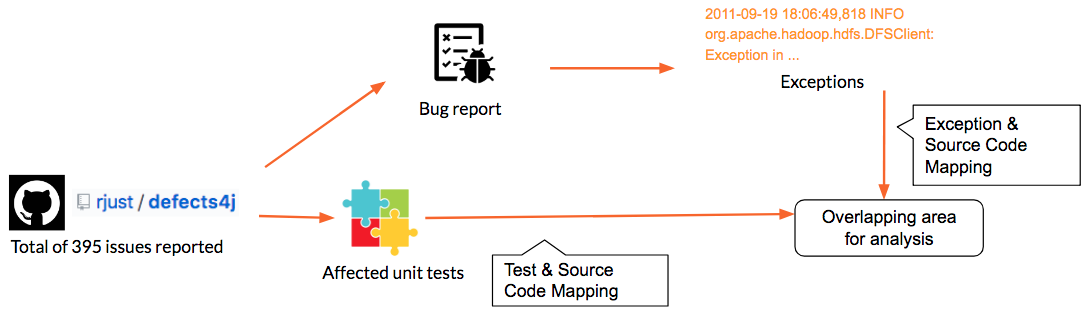
\includegraphics[width=\textwidth, height=5cm]{overview}
			\caption{Overview of the approach on test and exception mapping}
			\label{overview}
		\end{figure*}

		\begin{figure}[h]
			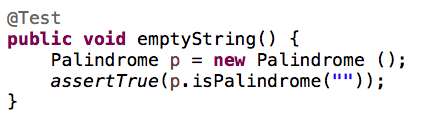
\includegraphics[width=0.4\textwidth,height=2cm]{test}
			\caption{emptyString() test case executed by JaCoCo}
			\label{test}
		\end{figure}

		\begin{figure}[h]
			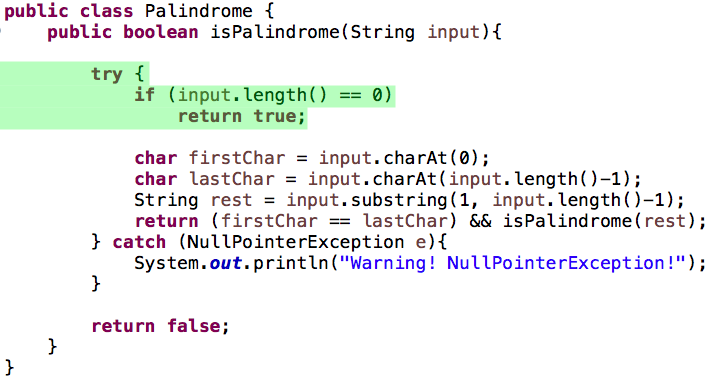
\includegraphics[width=0.5\textwidth]{jacoco}
			\caption{JaCoCo Test Coverage Mapping to Source Code}
			\label{jacoco}
		\end{figure}

		\begin{figure}[h]
			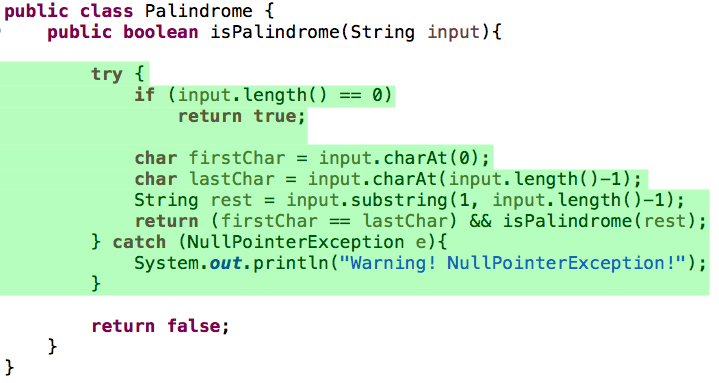
\includegraphics[width=0.5\textwidth]{exception_code_mapping}
			\caption{Exception and Source Code Mapping}
			\label{exception_code_mapping}
		\end{figure}

		\begin{figure}[h]
			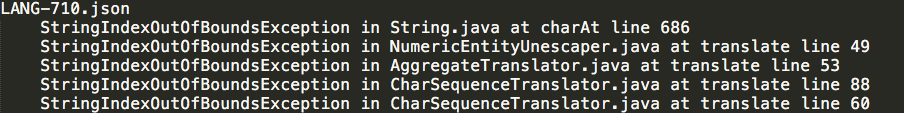
\includegraphics[width=0.5\textwidth]{list_calls_exception}
			\caption{Example of list of method calls extracted from the exception stack trace}
			\label{list_calls_exception}
		\end{figure}

		\phead{Overview of Our Approach} We match the exception stack trace with the related test cases based on the source code. First, from the exception stack trace, we pinpoint the location in code where the problem might have occured. Second, we map the source code to the test cases that cover it according to the test execution path. Lastly, we traverse the test execution path to find the corresponding log events that appear on the stack trace. Part of the stack trace may overlap with the test execution. Based on this overlapping, we analyze the correlation between tests and production failures, and discuss how could those failures contribute to better test cases. Figure \ref{overview} shows an overview of our approach.

		\phead{Exception and Source Code Mapping} Inside each bug report, we use regular regex to retrieve the exception stack trace. From there, we derive a list of method calls. An example of list of method calls is showed in Figure \ref{list_calls_exception}. Figure \ref{exception_code_mapping} illustrates the mapping between source code and a NullPointerException. Basically, we map everything that is inside the try-catch block.

		\phead{Test and Source Code Mapping} To identify the mapping between the test and source code, we use JaCoCo, a Java code coverage library. By running the individual unit test, the tool highlights the covered branches and generates a coverage report. We use the covered branches to identify the portion of code that have been called by the tests. This will later help us to observe the overlaps between the source code exercised in tests with the one executed by user-reported exceptions. In addition, in future research, we will analyze the metrics (e.g., instructions coverage, branches coverage and cyclomatic complexity) from the coverage report to conclude some generic findings on the characterics of codes that can easily be covered through a small modification in tests. Figure \ref{test} and \ref{jacoco} illustrates an example of test and source code mapping exercised by JaCoCo.

		\phead{Exception and test mapping} At last, we connect tests and exceptions that cover the same portion of the source code. 
	~\\

	\subsubsection{Result}~

		Unit tests need to ensure the correctness of the program execution, on top of which it should also guarantee that all runtime errors are handled properly during a normal execution flow. Error handling tests are necessary to verity that correct exceptions are caught when the system encounters unexpected behavious (e.g., runtime errors). In two out of the six bug reports that we have manually studied, we were able to confirm the underlying root cause of system failures was related to exception handling problems. Thus, we studied the number of \verb/catch/ statements that were covered by testing.

		We performed a regex search to find the tests that contain exception handling statements (e.g., \verb/catch\s*\(([a-zA-z.])*Exception/) or \textit{expected} parameter in \textit{@Test} annotation (e.g., \textit{@Test(expected = IndexOutOfBoundsException.class)}). Then, we run tests with JaCoCo to map the individual test case to the exceptions that are been covered.

		Across the Lang project, there are 96 exception handling statements. Based on the results, only 44 of them are tested, meaning that more than half of the handling statements remain untested. This translates to a poor reliability of the code. However, it might be hard to tell which of the statements absolutely need to be covered by testing. There could be many reasons why some handling statements are left untested intentionally by the developer. Thus, the finding also reflects some practical implications that we need to address: how can we highlight the vulnerable exception handling statements that need to be tested?

		\finding{\textbf{Finding 1}: \textit{Among the 96 exception handling statements, only 45.8\% are covered by unit test}}

		We propose an automated approach to detect the most vulnerable statements based on past development history. We need to know the types of exception that are most likely to cause critical system failure. There is a great amount of exception messages that could be collected from the project Jira issue tracker. Hence, we can extract a list of the most common exceptions using regular expression. We run the coverage tool in source code to obtain a list of exception handling statements that haven't been covered by any of the tests and mark them as \textit{vulnerable}. If the \textit{vulnerable} exception also appears to be one that often causes system failure, then we notify the developers. They will further investigate the statement and decide on adding an exception test. 

		In addition, to uncover the exception handling that were not previsouly tested, a deeper exception testing is necessary. For instance, we also suggest to check the value of the message in the exception (e.g., \textit{assertThat(expected.getMessage(), is("Index > Size"));}) for two reasons. First, the assertion checks that the exception is thrown under the right context. Second, it also encourages the developer to improve the quality of the exception message. The messages originated from the same type of exception should differentiate one from another because the different context in which they are used.

		\finding{\textbf{Finding 2}: \textit{Over-catching exceptions are bad for testing}}
 
		As a high-level exception can happen at any time in test execution, we wouldn't be able to tell where the exception is throw. We should always throw exception with feature related information. This provides a connection with the feature under test and help the tester to focus on a specific unit. To address this issue, we propose to implement a bug pattern to detect over-catching exception statements. 
	~\\

	\subsubsection{Open Research Findings}~

		\textbf{How much does the test case need to change to capture the problem?} 
		
		To answer this research question, we used the number of instructions modified as unit of evaluation to the amount of changes required. Across the six bug reports that we have manually studied, the repair was fairly easy in most of the time. It requires less than 10 lines of codes (LOC) to fix the bug. Although the effort to repair these issues was trivial, among 20 observed issues, the least development time required (the interval of time between the moment where the assignee first replies to the moment where a fix is commited) was five hours. Hence, to reduce the repair effort, we suggest to push this study further towards the automated program repair area. By varying the test execution path, we can generate new test cases that aim to fail the system. We would execise our approach in the less reliable portion of the code.

		Finding 1 motivates us to study the untested exceptions more closely. It would be interesting to investigate the nature of the untested exceptions. 

		\finding{\textbf{Finding 3}: \textit{Among the six manually studied reports, we calculate an average of 27 instructions coverage ( and an average of 4 methods coverage) improvement after a bug fix}} 
		
		\textbf{How could the test coverage metrics (e.g., branch coverage, instruction coverage) reflect the improvement of test cases? ( focusing on the reliability of tests)} We could measure the reliability of the tests after repair by two factors: 1. the improvement in coverage metrics 2. the likelihood of causing regression. With the coverage metrics, we calculated an average of 27 instructions coverage ( and an average of 4 methods coverage) improvement after a bug fix. The data might suggest there is an overall improvement since more instructions are been covered. However, it is also possible that the developer only covered the portion of the code that is new to the system in the bug fix. 
    ~\\
	
	\subsubsection{Limitations}~

		\textbf{Small sample set}. While we performed our study on 65 reported bugs, we have only selected six of them for our case studies. As there were not many issues that contain exceptions, we should have extracted the issues directly from Apache Commons Lang issues tracker. That is been said, we might have difficulties finding the related test cases from the user reports. We believe this research can act like a preliminary study for our future research. Ideally, we should have randomly sampled issues with a selection criteria that prevents duplicated bugs.

		\textbf{Representativeness of the seleted bugs}. We only studied bugs reported from Apache Commons Lang project. Some issues, such as misconfigurations, are project-related, which might not provide a generic finding for future research. In consequence, we only list common findings that can also be observed in other Java projects. 

		We do our best to categorize production errors into findings to better reflect the characteristics of distinct errors. 
	~\\